\documentclass[12pt]{amsart}
\usepackage{amsmath,amsthm,amssymb,mathrsfs,amsfonts,verbatim,enumitem,color,leftidx}
\usepackage{tikz}
\usepackage[colorlinks]{hyperref}
\usepackage{tikz}
\usetikzlibrary{arrows,snakes,backgrounds}

\begin{document}

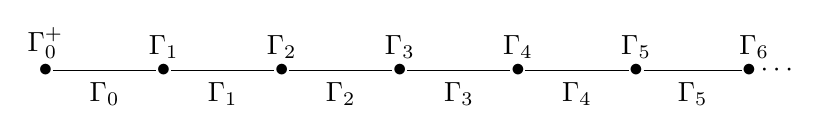
\begin{tikzpicture}[every loop/.style={}]
  \tikzstyle{every node}=[inner sep=0pt]
  \node (0) {$\bullet$} node [above=4pt] at (0,0) {$\Gamma_0^+$};
  \node (2) at (1.5,0) {$\bullet$} node [above=4pt] at (1.5,0) {$\Gamma_1$}; 
  \node (4) at (3,0) {$\bullet$}node [above=4pt] at (3,0) {$\Gamma_2$}; 
  \node (6) at (4.5,0) {$\bullet$}node [above=4pt] at (4.5,0) {$\Gamma_3$}; 
  \node (8) at (6,0) {$\bullet$}node [above=4pt] at (6,0) {$\Gamma_4$}; 
  \node (10) at (7.5,0) {$\bullet$}node [above=4pt] at (7.5,0) {$\Gamma_5$}; 
  \node (11) at (9.2,0) {$\bullet \cdots$}node [above=4pt] at (9,0) {$\Gamma_6$}; 

  \path[-] (0) edge node [below=4pt] {$\Gamma_0$} (2)
 (2) edge node [below=4pt] {$\Gamma_1$} (4)
(4) edge node [below=4pt] {$\Gamma_2$} (6)
 (6) edge node [below=4pt] {$\Gamma_3$} (8)
 (8) edge node [below=4pt] {$\Gamma_4$} (10)
 (10) edge node [below=4pt] {$\Gamma_5$} (11);
\end{tikzpicture}

\end{document}